\documentclass[a4paper,11pt]{article}

\usepackage[spanish]{babel}
\usepackage[utf8]{inputenc}
\usepackage{hyperref}
\usepackage{graphicx}
\usepackage{amsmath}
\graphicspath{{images/}} 

\author{Daniel Monjas Miguélez}
\title{FR: Tema 2}

\begin{document}
\begin{titlepage}
\centering
    \vfill
    {\bfseries\Large
        Fundamentos de Bases de Datos: Tema 1\\
        28 de Noviembre del 2020\\
        A year to Forget \\
        \vskip2cm
        Daniel Monjas Miguélez\\
    }    
    \vfill
    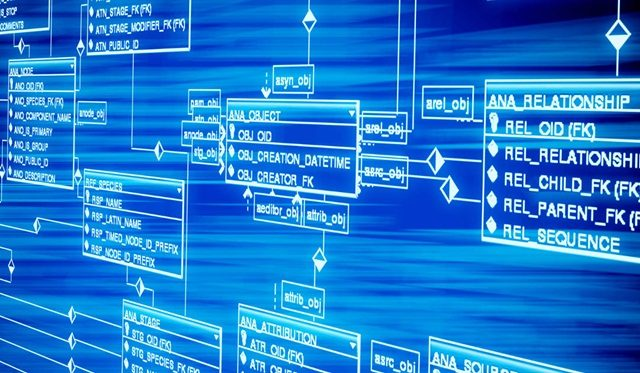
\includegraphics[width=13cm]{bases_datos.jpg}
    \vfill
    \vfill
\end{titlepage}

\newpage
\tableofcontents
\newpage

\section{Definiciones:}
\begin{itemize}
\item \textbf{Base de datos:} conjunto de datos comunes a un "proyecto" almacenados sin redundancia para ser útiles a diferentes aplicaciones.

\item \textbf{SGDB (Sistema de Gestión de Bases de Datos):} Conjunto de elementos software con capacidad de definir, mantener y utilizar una base de datos. Un SGBD debe permitir:
	\begin{itemize}
		\item Definir estructuras de almacenamiento.
		\item Acceder a los datos de forma eficiente y segura.
		\item Organizar la actualización de los datos y el acceso multiusuario
	\end{itemize}
\end{itemize}

\section{Sistema de Gestión de Base de Datos:}
Los elementos de una Base de Datos son:

\begin{itemize}
\item Datos
	\begin{itemize}
		\item Integrados(sin redundancia).
		\item Compartidos(útiles a varias aplicaciones).
	\end{itemize}
\item Hardware
	\begin{itemize}
		\item BD normal.
		\item BD distribuida (BDD): es un conjunto de múltiples bases de datos lógicamente relacionadas las cuales se encuentran distribuidas en diferentes espacios lógicos y geográficos e interconectados por una red de comunicaciones. Dichas BDD tienen la capacidad de realizar procesamientos autónomos, estos permiten realizar operaciones locales o distribuidas.
	\end{itemize}
\item Software(SGBD)
	\begin{itemize}
		\item Programas para definir las estructuras y gestionar la información de la BD.
	\end{itemize}

\item Usuarios
	\begin{itemize}
		\item Usuario final
		\item Programador de aplicaciones.
		\item Administrador (DBA,DBM).
	\end{itemize}
\end{itemize}

\textbf{Dato operativo:} es una pieza de información que necesita una organización para su funcionamiento, pueden ser:

\begin{itemize}
\item \textbf{Item básico:} elementos acerca de los que se puede pedir información (sustantivo).
\item \textbf{Atributos:} características de los ítem básicos (adjetivos).
\item \textbf{Relaciones:} conexiones lógicas entre ítems.
\end{itemize}

Cuando se determinan y clasifican de esta forma todos los datos operativos, se obtiene el esquema lógico de la Base de Datos.

\begin{figure}[h]
\centering
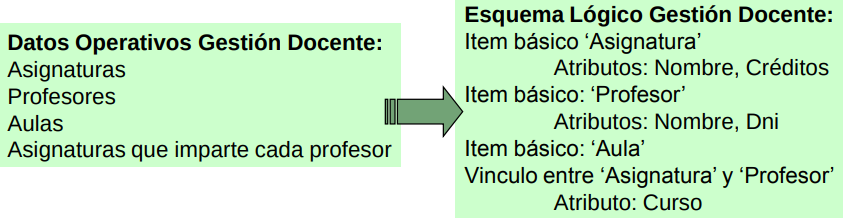
\includegraphics[scale=1,width=1.1\textwidth]{ejemplo_dato_operativo.png}
\caption{Ejemplo de datos operativo y del esquema lógico obtenido a partir de el.}
\end{figure}

\textbf{Objetivos de un SGBD:}
\begin{itemize}
\item \textbf{Independencia de los datos}: los datos se organizan independientemente de las aplicaciones que los vayan a usar y de los ficheros en los que vayan a almacenarse. Esta independencia puede ser:
	\begin{itemize}
		\item \textbf{Independencia física:} el diseño lógico de la BD, a todos los niveles debe ser independiente del almacenamiento físico de los datos. Esto permite realizar cambios en la estructura física sin alterar la lógica de la aplicación y descargar a las aplicaciones de gestionar los aspectos relativos al almacenamiento.
		
		\item \textbf{Independencia lógica:} existen dos tipos de estructuras lógicas, el esquema lógico general y las vistas de usuario. Cada aplicación debe poder organizar los datos según sus propios esquemas y acceder a los datos que le son necesarios y le conciernen. La independencia lógica persigue que los cambios en el esquema lógico general no afecten a las vistas de usuario de manera que las aplicaciones no necesiten ser modificadas (no siempre se puede conseguir). Si se consigue se produce un aumento de la seguridad y la fiabilidad, menos problemas para las aplicaciones y la posibilidad de cambios en los esquemas por parte de las aplicaciones y por parte de los administradores.
	\end{itemize}
\item \textbf{Diseño y utilización orientada al usuario}: Los datos y aplicaciones deben ser accesibles a los usuarios de la manera más amigable posible.
		
	\begin{itemize}
		\item Soportar un modelo de datos teórico
		\item Soportar facilidades de definición
		\item Soportar lenguajes de acceso y modificación
	\end{itemize}
\item \textbf{Centralización}: los datos deben gestionarse de forma centralizada e independiente de las aplicaciones. Para ello surge la figura del Administrador de Bases de Datos (DBA Data Base Administrator) y las utilidades de gestión.

\item \textbf{No redundancia:} los datos no deben estar duplicados (gratuitamente). Hay que asegurar la gestión de datos concurrentes.

\item \textbf{Consistencia:} los datos deben ser consistentes (sin fallo lógicos). Para ello deben haber mecanismo de mantenimiento de integridad y cada operación debe llevar a la BD de un estado válido a otro.

\item \textbf{Fiabilidad:} Los datos deben estar protegidos contra fallos catastróficos. Mecanismos de mantenimiento de recuperación y relanzamiento de transacciones.

\item \textbf{Seguridad:} No todos los datos deben ser accesibles a todos los usuarios. Deben de haber mecanismos de gestión de usuarios y privilegiso y mecanismo de protección de información.
\end{itemize}

\section{Ventajas de utilizar un SGBD}
\begin{itemize}
\item Ventajas para el usuario:

	\begin{itemize}
		\item Al usuario final le permite acceder a los datos.
		\item Al programador de aplicaciones le elimina problemas de diseño lógico y físico, depuración de errores y mantenimiento en general (copias de seguridad, recuperación de fallos, etc.).
		\item Con la aparición de las Bases de Datos surge la figura del administrador de Bases de Datos.
	\end{itemize}
	
\item Ventajas para el sistema:
	
	\begin{itemize}
		\item Permite un control centralizado: fiabilidad, consistencia, seguridad...
		\item Escalabilidad: a nivel de capacidad de procesamiento y rendimiento.
		\item Criterios de uniformización.
		\item Generación de nuevas aplicaciones.
		\item Equilibrio entre requerimentos conflictivos.
	\end{itemize}
\end{itemize}


\end{document}